\documentclass[aspectratio=169,10pt]{beamer}

% Theme and typography
\usetheme{Madrid}
\usecolortheme{seahorse}

\definecolor{navyblue}{RGB}{20, 45, 85}
\definecolor{accentteal}{RGB}{0, 130, 140}
\definecolor{alertred}{RGB}{180, 40, 40}
\definecolor{lightbg}{RGB}{245, 247, 250}

\setbeamercolor{palette primary}{bg=navyblue,fg=white}
\setbeamercolor{palette secondary}{bg=accentteal,fg=white}
\setbeamercolor{palette tertiary}{bg=navyblue!90,fg=white}
\setbeamercolor{structure}{fg=navyblue}
\setbeamercolor{titlelike}{parent=palette primary}
\setbeamercolor{block title}{bg=navyblue!15,fg=navyblue}
\setbeamercolor{block body}{bg=lightbg,fg=black}
\setbeamercolor{block title alerted}{bg=alertred!15,fg=alertred}
\setbeamercolor{block body alerted}{bg=lightbg,fg=black}
\setbeamercolor{block title example}{bg=accentteal!15,fg=accentteal}
\setbeamercolor{block body example}{bg=lightbg,fg=black}

\usepackage{amsmath,amssymb,amsfonts,amsthm}
\usepackage{booktabs}
\usepackage{multirow}
\usepackage{graphicx}
\usepackage{tikz}
\usepackage{algorithm}
\usepackage{algpseudocode}

\title[AURA-HOI: Exact HOI Mining on Dense Databases]{AURA-HOI: Exact High-Occupancy Itemset Mining on Dense Databases with a Length-Capped Residual Bound}
\subtitle{Theory, Mathematical Dominance, Systems Architecture \& Empirical Audit}
\author[Q.~Van]{Q.~Van}
\institute[JIIS 2026]{
  Journal of Intelligent Information Systems (JIIS)\\
  Springer Nature
}
\date{October 2026}

\newcommand{\AURA}{\textsc{AURA-HOI}}
\newcommand{\HEP}{\textsc{HEP}}
\newcommand{\DFHOI}{\textsc{DFHOI}}
\newcommand{\supp}{\operatorname{supp}}
\newcommand{\occ}{\operatorname{occ}}
\newcommand{\UBO}{\operatorname{UBO}}
\newcommand{\UBres}{\operatorname{UB}_{\text{res}}}
\newcommand{\tail}{\operatorname{tail}}
\newcommand{\Subtree}{\operatorname{Subtree}}

\begin{document}

% Slide 1: Title
\begin{frame}[plain]
  \titlepage
\end{frame}

% Slide 2: Outline
\begin{frame}{Table of Contents}
  \tableofcontents
\end{frame}

% ==============================================================================
% SECTION 1: PROBLEM FORMULATION & MOTIVATION
% ==============================================================================
\section{Motivation \& Problem Formulation}

\begin{frame}{Context: Why Frequent Itemset Mining (FIM) Fails}
  \begin{itemize}
    \item \textbf{Frequent Itemset Mining (FIM):} Measures frequency across transactions ($\supp(X) \ge \theta$).
    \item \textbf{The Dilution Paradox in Large/Dense Baskets:}
      \begin{itemize}
        \item A pair $\{A, B\}$ appearing in $10,000$ transactions of size $500$ has high support ($10,000$).
        \item Yet, $\{A, B\}$ represents a mere $\frac{2}{500} = 0.4\%$ of each basket content!
        \item Downstream applications (recommendation, bundle pricing, clinical diagnosis) mistakenly treat dilute artifacts as core customer behaviors.
      \end{itemize}
    \item \textbf{High-Occupancy Itemsets (HOI) [Deng, 2020]:}
      \begin{itemize}
        \item Constrains patterns to physically \textbf{dominate} the transactions containing them.
        \item Occupancy balances recurrence with within-transaction density.
      \end{itemize}
  \end{itemize}

  \begin{block}{Core Objective}
    Mine all item combinations whose average relative contribution across the transaction database meets or exceeds a user-defined threshold $\alpha$.
  \end{block}
\end{frame}

\begin{frame}{Formal Problem Definition}
  \begin{definition}[Database, Support \& Occupancy]
    Let $\mathcal{D} = \{t_1, \dots, t_n\}$ be a database over item alphabet $\mathcal{I}$. For an itemset $X \subseteq \mathcal{I}$:
    \begin{itemize}
      \item \textbf{Supporting Transactions:} $T(X) = \{t_q \in \mathcal{D} \mid X \subseteq t_q\}$, and $\supp(X) = |T(X)|$.
      \item \textbf{Transaction Occupancy:} $\occ(X, t_q) = \frac{|X|}{|t_q|}$ if $t_q \in T(X)$, else $0$.
      \item \textbf{Global Occupancy:} Average coverage across the entire database:
      $$\occ(X) \triangleq \frac{1}{|\mathcal{D}|} \sum_{t_q \in T(X)} \frac{|X|}{|t_q|} = \frac{|X|}{|\mathcal{D}|} \sum_{t_q \in T(X)} \frac{1}{|t_q|}$$
    \end{itemize}
  \end{definition}

  \begin{block}{The HOI Mining Problem}
    Given database $\mathcal{D}$ and threshold $\alpha \in (0, 1]$, discover the complete set of High-Occupancy Itemsets:
    $$\mathcal{H} \triangleq \{X \subseteq \mathcal{I} \mid \occ(X) \ge \alpha\}$$
  \end{block}
\end{frame}

\begin{frame}{The Dual Non-Monotonicity Dilemma}
  \begin{alertblock}{Anti-Monotonicity Fails for Occupancy}
    In FIM, if $X \subseteq Y$, then $\supp(X) \ge \supp(Y)$ (Apriori downward-closure property).
    \textbf{For occupancy, this monotonicity strictly fails!}
  \end{alertblock}

  \vspace{0.3cm}
  Consider appending an item $e$ to $X$, yielding $Y = X \cup \{e\}$:
  \begin{itemize}
    \item \textbf{Numerator Effect ($\uparrow$):} Cardinality increases from $|X|$ to $|X| + 1$, increasing the fractional factor $\frac{|X|+1}{|t_q|}$.
    \item \textbf{Denominator Effect ($\downarrow$):} Supporting transaction set shrinks: $T(Y) \subseteq T(X)$.
  \end{itemize}

  \begin{exampleblock}{Concrete Divergence}
    \begin{itemize}
      \item $X = \{A\}$ in $t_1 = \{A, B, C\}$ ($|t_1|=3$): $\occ(X) = \frac{1}{3} \approx 0.333$.
      \item $Y = \{A, B\}$ in $t_1 = \{A, B, C\}$: $\occ(Y) = \frac{2}{3} \approx 0.667 > \occ(X)$! (Superset has \textbf{higher} occupancy).
      \item $Z = \{A, B, D\}$ in $t_1$: $t_1 \notin T(Z) \implies \occ(Z) = 0$ (Drop to zero).
    \end{itemize}
  \end{exampleblock}
  $\implies$ \textbf{Pruning requires sound, tight mathematical upper bounds over all potential descendants.}
\end{frame}

\begin{frame}{State of the Art: The Transaction-Length Bound (UBO)}
  Existing exact miners (\HEP{} [Deng, 2020] and \DFHOI{} [Nguyen et al., 2023]) establish an upper bound by assuming every descendant $Y \supseteq X$ can grow up to the entire size of each supporting transaction:
  
  \begin{block}{Transaction-Length Upper Bound ($\UBO$)}
    $$\occ(Y, t_q) \le \frac{|t_q|}{|t_q|} = 1 \implies \UBO(X) \triangleq \frac{1}{|\mathcal{D}|} \sum_{t_q \in T(X)} \frac{|t_q|}{|t_q|} = \frac{|T(X)|}{|\mathcal{D}|} = \frac{\supp(X)}{|\mathcal{D}|}$$
  \end{block}

  \begin{alertblock}{Critical Vulnerability on Dense Databases}
    \begin{itemize}
      \item In dense databases (e.g., \texttt{mushroom}, \texttt{accidents}, \texttt{chess}, \texttt{pumsb}), transactions are long ($|t_q| \in [23, 74]$) and item co-occurrence is very high.
      \item $\UBO(X)$ becomes equal or nearly equal to relative support.
      \item \textbf{Combinatorial Explosion:} $\UBO(X)$ grossly overestimates occupancy, forcing miners to generate millions of fruitless candidates and perform expensive TID-list intersections.
    \end{itemize}
  \end{alertblock}
\end{frame}

% ==============================================================================
% SECTION 2: THE NOVEL LENGTH-CAPPED RESIDUAL BOUND
% ==============================================================================
\section{The Length-Capped Residual Bound}

\begin{frame}[fragile]{Key Geometric Insight: Search-Tree Length Capping}
  \begin{columns}[T]
    \begin{column}{0.55\textwidth}
      \begin{itemize}
        \item In a depth-first search tree with a fixed item ordering $\prec$, node $X$ is extended only by items from its candidate tail:
        $$\tail(X) = \{e \in \mathcal{I} \mid e \succ \max(X) \text{ and } \supp(X \cup \{e\}) \ge 1\}$$
        \item Any descendant $Y \in \Subtree(X)$ can contain \textbf{at most} all items of $X$ plus all items in $\tail(X)$:
        $$|Y| \le L(X) \triangleq |X| + |\tail(X)|$$
        \item \textbf{Key Observation on Dense Data:}
        Deep in the search tree, $|\tail(X)|$ shrinks rapidly, causing $L(X) \ll |t_q|$ for almost all supporting transactions!
      \end{itemize}
    \end{column}
    \begin{column}{0.42\textwidth}
      \begin{block}{The Structural Ceiling}
        \centering
        \vspace{0.2cm}
        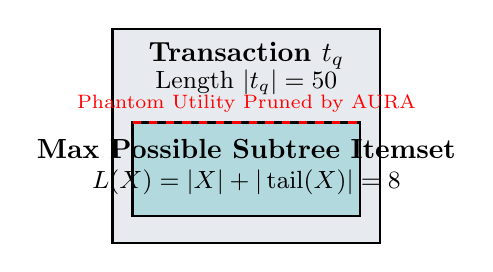
\begin{tikzpicture}[scale=0.85]
          \draw[thick, fill=navyblue!10] (0,0) rectangle (4, 3.2);
          \node at (2, 2.8) {\textbf{Transaction $t_q$}};
          \node at (2, 2.4) {\small Length $|t_q| = 50$};
          
          \draw[thick, fill=accentteal!30] (0.3, 0.4) rectangle (3.7, 1.8);
          \node at (2, 1.4) {\textbf{Max Possible Subtree Itemset}};
          \node at (2, 0.9) {\small $L(X) = |X| + |\tail(X)| = 8$};
          
          \draw[dashed, red, thick] (0.3, 1.8) -- (3.7, 1.8);
          \node[red, above] at (2, 1.8) {\scriptsize Phantom Utility Pruned by AURA};
        \end{tikzpicture}
      \end{block}
      \end{column}
  \end{columns}
\end{frame}

\begin{frame}{The Length-Capped Residual Bound: Formulation}
  \begin{definition}[Length-Capped Residual Bound $\UBres(X)$]
    Let $X$ be an itemset in the DFS tree with supporting transaction set $T(X)$ and maximum reachable descendant cardinality $L(X) = |X| + |\tail(X)|$. The length-capped residual bound is:
    $$\UBres(X) \triangleq \frac{1}{|\mathcal{D}|} \sum_{t_q \in T(X)} \min\left(1, \frac{L(X)}{|t_q|}\right)$$
  \end{definition}

  \begin{block}{Decomposition into Two Regimes}
    For each supporting transaction $t_q \in T(X)$:
    \begin{enumerate}
      \item If $|t_q| \le L(X)$: The transaction is short; occupancy could theoretically reach $1$. Contribution: $1$.
      \item If $|t_q| > L(X)$: The transaction is long; occupancy can \textbf{never} exceed $\frac{L(X)}{|t_q|} < 1$. Contribution: $\frac{L(X)}{|t_q|}$.
    \end{enumerate}
  \end{block}
  $$\implies \UBres(X) = \frac{1}{|\mathcal{D}|} \left( \sum_{t_q \in T(X), |t_q| \le L(X)} 1 + L(X) \sum_{t_q \in T(X), |t_q| > L(X)} \frac{1}{|t_q|} \right)$$
\end{frame}

\begin{frame}{Theoretical Foundation: Soundness \& Dominance}
  \begin{block}{Lemma 1 (Soundness / Upper Bound Guarantee)}
    For every itemset $X$ and every descendant $Y \in \Subtree(X)$, $\occ(Y) \le \UBres(X)$.
  \end{block}
  \begin{proof}[Proof Sketch]
    Let $Y \in \Subtree(X)$. By definition of the DFS tail, $Y \subseteq X \cup \tail(X)$, so $|Y| \le L(X)$.
    Also, $T(Y) \subseteq T(X)$. For every $t_q \in T(Y)$, $\occ(Y, t_q) = \frac{|Y|}{|t_q|} \le \frac{L(X)}{|t_q|}$, and trivially $\occ(Y, t_q) \le 1$.
    Thus, $\occ(Y, t_q) \le \min\left(1, \frac{L(X)}{|t_q|}\right)$. Summing over $T(Y) \subseteq T(X)$ and dividing by $|\mathcal{D}|$ yields $\occ(Y) \le \UBres(X)$.
  \end{proof}

  \begin{block}{Lemma 2 (Strict Dominance over $\UBO$)}
    For all itemsets $X$, $\UBres(X) \le \UBO(X)$. Furthermore, if $\exists t_q \in T(X)$ such that $|t_q| > L(X)$, then the inequality is \textbf{strictly tighter}: $\UBres(X) < \UBO(X)$.
  \end{block}
  \begin{proof}
    $\min\left(1, \frac{L(X)}{|t_q|}\right) \le 1$ for every $t_q$. Hence $\sum \min(1, \frac{L}{|t_q|}) \le |T(X)|$. When $|t_q| > L(X)$, $\frac{L(X)}{|t_q|} < 1$, eliminating a positive surplus $\delta_q = 1 - \frac{L(X)}{|t_q|}$.
  \end{proof}
\end{frame}

\begin{frame}{Characterization Theorem: Pruning Scope}
  \begin{theorem}[Exact Scope of Dominance]
    $\UBres(X) = \UBO(X)$ if and only if for all supporting transactions $t_q \in T(X)$, $|t_q| \le L(X)$.
  \end{theorem}

  \begin{block}{Practical Consequence}
    \begin{itemize}
      \item \textbf{Dense Databases:} Transactions have large lengths (e.g., $|t_q| \approx 30$--$75$). At moderate depth in the search tree, $|\tail(X)|$ falls below $20$, making $|t_q| > L(X)$ hold for \textbf{nearly 100\%} of supporting transactions. $\implies$ Massive, exponential pruning!
      \item \textbf{Sparse Databases:} Transactions are short ($|t_q| \approx 8$--$10$), while alphabet $\mathcal{I}$ is large ($|\tail(X)| \approx 1000$). Here $L(X) \gg |t_q|$, so $\UBres(X)$ smoothly reduces to $\UBO(X)$ without correctness penalty.
    \end{itemize}
  \end{block}

  \begin{alertblock}{No False Dismissals}
    Because $\UBres(X)$ is a mathematically proven upper bound for all descendants, pruning any branch where $\UBres(X) < \alpha$ guarantees \textbf{zero false dismissals} (100\% exactness).
  \end{alertblock}
\end{frame}

\begin{frame}{Optimization: Uniform-Length Closed Form}
  \begin{proposition}[$O(1)$ Bound Evaluation on Uniform Databases]
    If all transactions in $\mathcal{D}$ have the identical length $M$ (as in standard benchmarks \texttt{mushroom} ($M=23$), \texttt{chess} ($M=37$), and \texttt{pumsb} ($M=74$)), then for any itemset $X$:
    $$\UBres(X) = \min\left(1, \frac{L(X)}{M}\right) \cdot \frac{\supp(X)}{|\mathcal{D}|}$$
  \end{proposition}

  \begin{block}{Computational Significance}
    \begin{itemize}
      \item Completely eliminates the $O(|T(X)|)$ iteration loop over supporting transactions.
      \item Evaluated in $O(1)$ arithmetic operations prior to performing candidate intersections!
      \item If $\min\left(1, \frac{L(X)}{M}\right) \cdot \supp(X) < \alpha \cdot |\mathcal{D}|$, the entire subtree is pruned \textbf{instantaneously}.
    \end{itemize}
  \end{block}
\end{frame}

% ==============================================================================
% SECTION 3: SYSTEM ARCHITECTURE & OPTIMIZATIONS
% ==============================================================================
\section{Algorithmic Architecture \& Systems Design}

\begin{frame}[fragile]{The \AURA{} Algorithm: DFS with Equivalence Classes}
  \begin{algorithm}[H]
    \caption{\AURA{} Recursive Mining Procedure}
    \begin{algorithmic}[1]
      \Procedure{MineSubtree}{$X, \operatorname{Candidates}, \alpha, \mathcal{D}$}
        \State $L \gets |X| + |\operatorname{Candidates}|$
        \State \Comment{\textbf{Rule 1: Length-Capped Residual Bound Check}}
        \If{$\UBres(X, L, \mathcal{D}) < \alpha$} \Return \EndIf
        \ForAll{$i \in \operatorname{Candidates}$}
          \State $Y \gets X \cup \{i\}$; \quad $T(Y) \gets T(X) \cap T(i)$ \Comment{Bitset/TID-list Intersection}
          \State \Comment{\textbf{Rule 2: Transaction-Length / Support Check}}
          \If{$\supp(Y) / |\mathcal{D}| < \alpha$} \textbf{continue} \EndIf
          \State \Comment{\textbf{Exact Evaluation \& Emission}}
          \If{$\occ(Y) \ge \alpha$} \State \textbf{output} $Y$ \EndIf
          \State $\operatorname{NewCand} \gets \{j \in \operatorname{Candidates} \mid j \succ i \text{ and } T(Y) \cap T(j) \neq \emptyset\}$
          \State \Call{MineSubtree}{$Y, \operatorname{NewCand}, \alpha, \mathcal{D}$}
        \EndFor
      \EndProcedure
    \end{algorithmic}
  \end{algorithm}
\end{frame}

\begin{frame}{Exact Rational Arithmetic Kernel}
  \begin{alertblock}{The Peril of IEEE 754 Floating-Point Comparison}
    \begin{itemize}
      \item Accumulating thousands of terms $\frac{|X|}{|t_q|}$ introduces numerical drift: $(1/3 + 1/3 + 1/3) \neq 1.0$.
      \item Near boundary cases ($\occ(X) \approx \alpha$), miners using floating-point can either spuriously discard true HOIs or admit invalid patterns.
    \end{itemize}
  \end{alertblock}

  \begin{block}{Exact Rational Decision in \AURA{} (\texttt{dm\_exact\_occ.h})}
    \begin{itemize}
      \item When $\alpha$ is rational $\frac{p}{q}$, the threshold condition $\frac{|X|}{|\mathcal{D}|} \sum_{q} \frac{1}{|t_q|} \ge \frac{p}{q}$ is rewritten as:
      $$q \cdot |X| \cdot \sum_{t_q \in T(X)} \frac{\operatorname{LCM}(\{|t_q|\})}{|t_q|} \ge p \cdot |\mathcal{D}| \cdot \operatorname{LCM}(\{|t_q|\})$$
      \item Fast-path double comparison outside an exact $\epsilon$-tolerance band; switches to exact bignum rational integer comparison inside the band.
      \item \textbf{Guarantees 100\% mathematical parity and bit-exact reproducibility.}
    \end{itemize}
  \end{block}
\end{frame}

\begin{frame}{Chunked Arena Memory Architecture}
  \begin{columns}[T]
    \begin{column}{0.5\textwidth}
      \begin{block}{Problem with Dynamic Allocations}
        \begin{itemize}
          \item Classical miners allocate TID-lists via individual \texttt{malloc()}/\texttt{free()} calls or Java objects.
          \item In dense trees with millions of nodes, this causes:
            \begin{itemize}
              \item Catastrophic heap fragmentation.
              \item High CPU overhead in allocator locks.
              \item Poor cache locality.
            \end{itemize}
        \end{itemize}
      \end{block}
    \end{column}
    \begin{column}{0.5\textwidth}
      \begin{block}{\AURA{} Chunked Arena Allocator}
        \begin{itemize}
          \item Pre-allocates large, contiguous memory slabs (chunks of 4--16 MiB).
          \item Allocation is a pointer bump:
          $$\text{ptr} = \text{arena.top}; \quad \text{arena.top} += \text{size};$$
          \item Recursion unwind: Entire tree level released instantaneously by restoring $\text{top}$ pointer.
          \item \textbf{Yields up to 22\% runtime reduction on dense datasets!}
        \end{itemize}
      \end{block}
    \end{column}
  \end{columns}
\end{frame}

% ==============================================================================
% SECTION 4: EXPERIMENTAL EVALUATION
% ==============================================================================
\section{Empirical Evaluation \& Experimental Audit}

\begin{frame}{Experimental Protocol \& Benchmark Datasets}
  \begin{columns}[T]
    \begin{column}{0.52\textwidth}
      \begin{block}{Standard Benchmark Datasets (SPMF/FIMI)}
        \begin{table}
          \scriptsize
          \setlength{\tabcolsep}{2pt}
          \begin{tabular}{llrrrr}
            \toprule
            Dataset & Type & $n$ & $|\mathcal{I}|$ & Avg.\ Len & Density \\
            \midrule
            \texttt{mushroom} & Dense & 8,416 & 119 & 23.0 & 19.33\% \\
            \texttt{accidents} & Dense & 340,183 & 468 & 33.8 & 7.22\% \\
            \texttt{chess} & Dense & 3,196 & 75 & 37.0 & 49.33\% \\
            \texttt{pumsb} & Dense & 49,046 & 2,113 & 74.0 & 3.50\% \\
            \midrule
            \texttt{retail} & Sparse & 88,162 & 16,470 & 10.3 & 0.06\% \\
            \texttt{kosarak} & Sparse & 990,002 & 41,270 & 8.1 & 0.02\% \\
            \texttt{T10I4D100K} & Sparse & 100,000 & 870 & 10.1 & 1.16\% \\
            \bottomrule
          \end{tabular}
        \end{table}
      \end{block}
    \end{column}
    \begin{column}{0.45\textwidth}
      \begin{block}{Rigorous Setup}
        \begin{itemize}
          \item \textbf{Hardware:} Intel Core i7-10700 (2.9--4.8 GHz), 32 GiB DDR4 RAM, Ubuntu 24.04 LTS.
          \item \textbf{Baselines:} \HEP{} [Deng 2020] and \DFHOI{} [Nguyen 2023], both implemented in optimized native C.
          \item \textbf{Execution Caps:} 600 s wall-clock time limit (TL), 20 GiB address space limit (ML).
          \item Single thread pinned with \texttt{taskset}.
        \end{itemize}
      \end{block}
    \end{column}
  \end{columns}
\end{frame}

\begin{frame}{RQ1: Pruning Efficacy (Candidate Intersections)}
  \begin{columns}[T]
    \begin{column}{0.48\textwidth}
      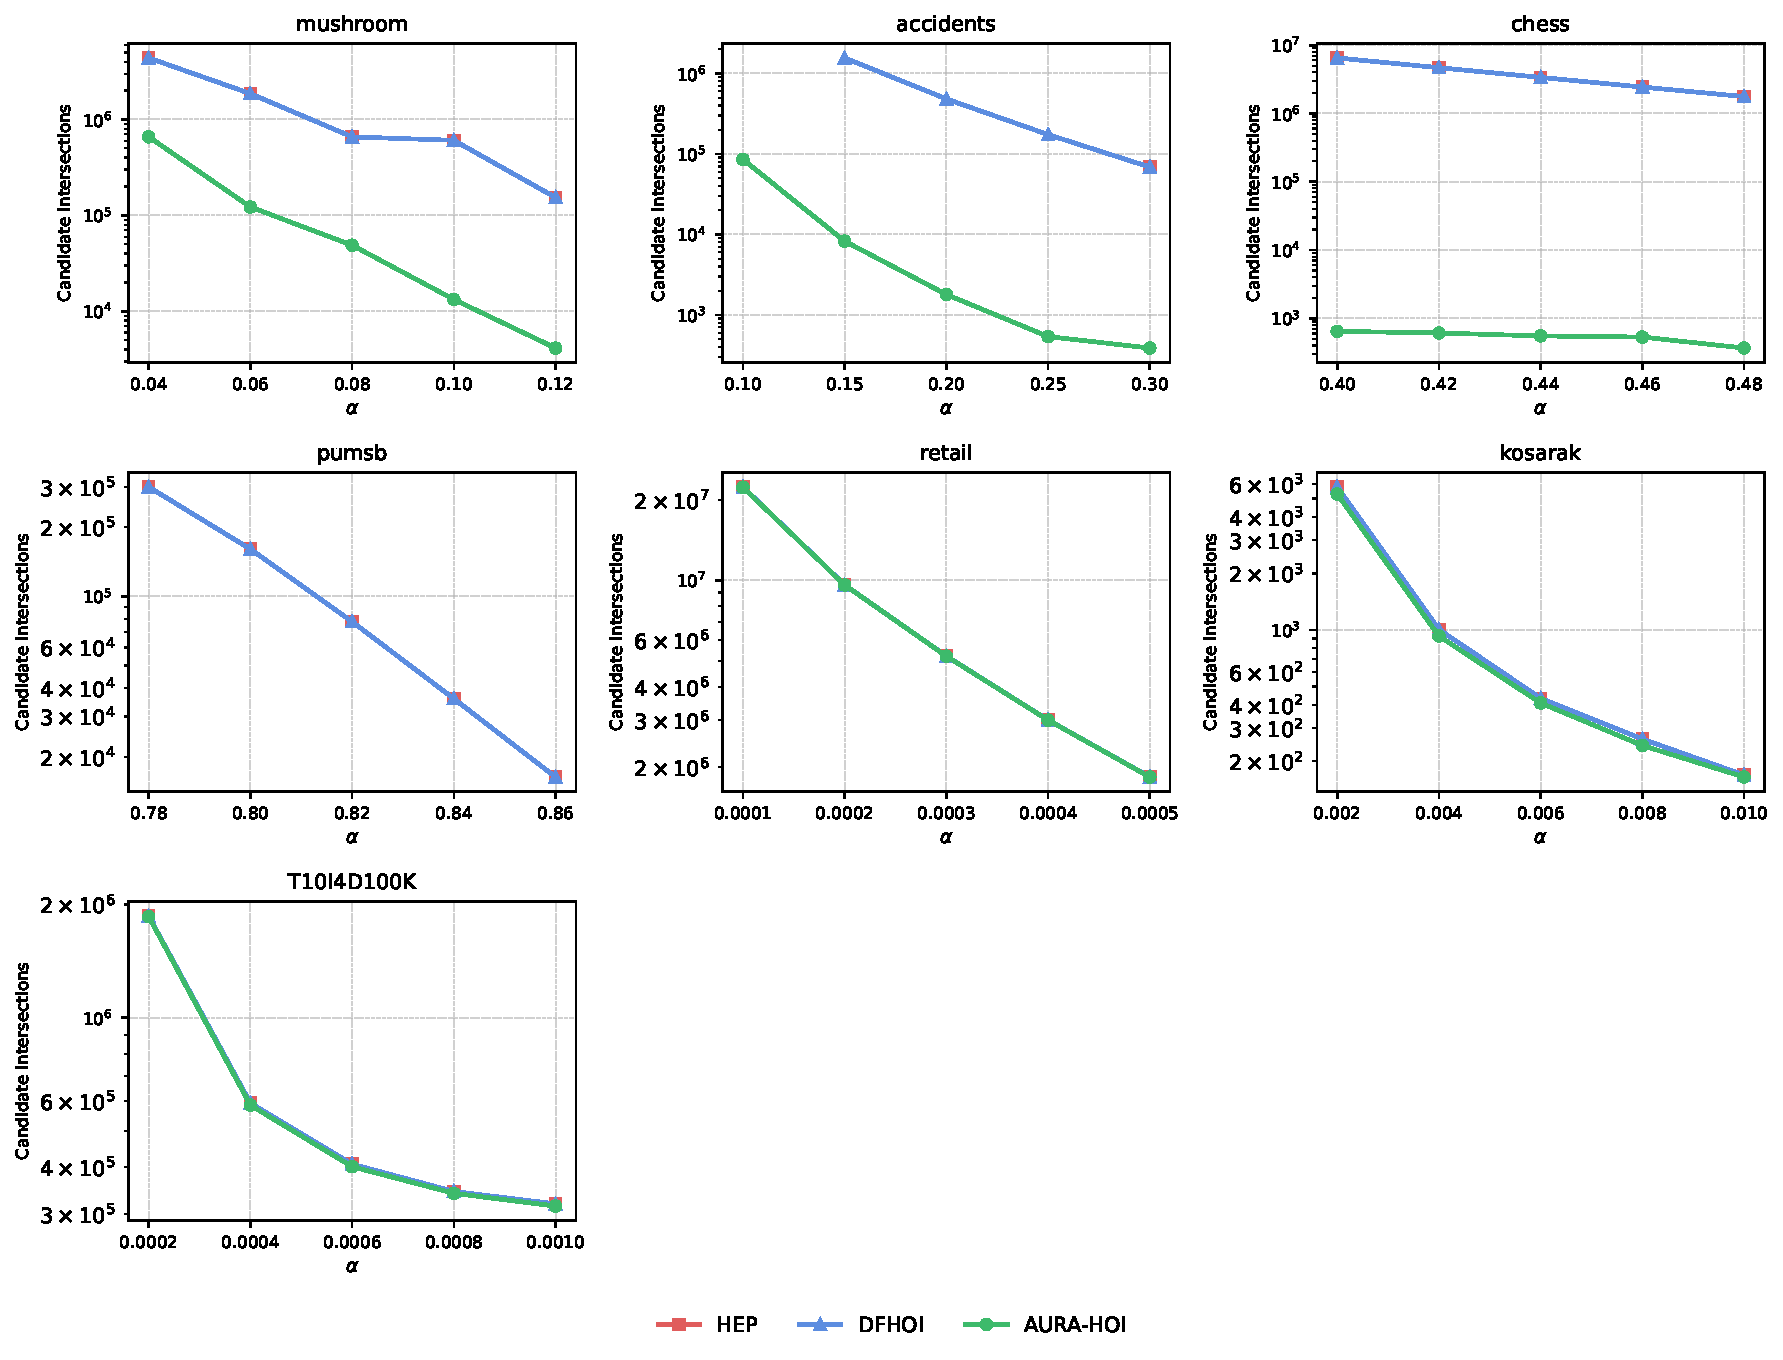
\includegraphics[width=\linewidth]{figures/nodes.pdf}
    \end{column}
    \begin{column}{0.48\textwidth}
      \begin{block}{Language-Independent Proof}
        \begin{itemize}
          \item Number of candidate intersections is an invariant metric of pure mathematical pruning tightness.
          \item \textbf{Dense Results:}
            \begin{itemize}
              \item \texttt{mushroom}: \textbf{93.4\%} node reduction over \DFHOI{}.
              \item \texttt{accidents}: \textbf{99.5\%} node reduction!
              \item \texttt{chess}: reduces intersections from $3.37 \times 10^6$ to 551 ($>99.98\%$).
              \item \texttt{pumsb}: reduces from $7.7 \times 10^4$ to 0.
            \end{itemize}
          \item Eliminates virtually all combinatorial exploration in dense search spaces!
        \end{itemize}
      \end{block}
    \end{column}
  \end{columns}
\end{frame}

\begin{frame}{RQ2: Runtime Efficiency}
  \begin{columns}[T]
    \begin{column}{0.48\textwidth}
      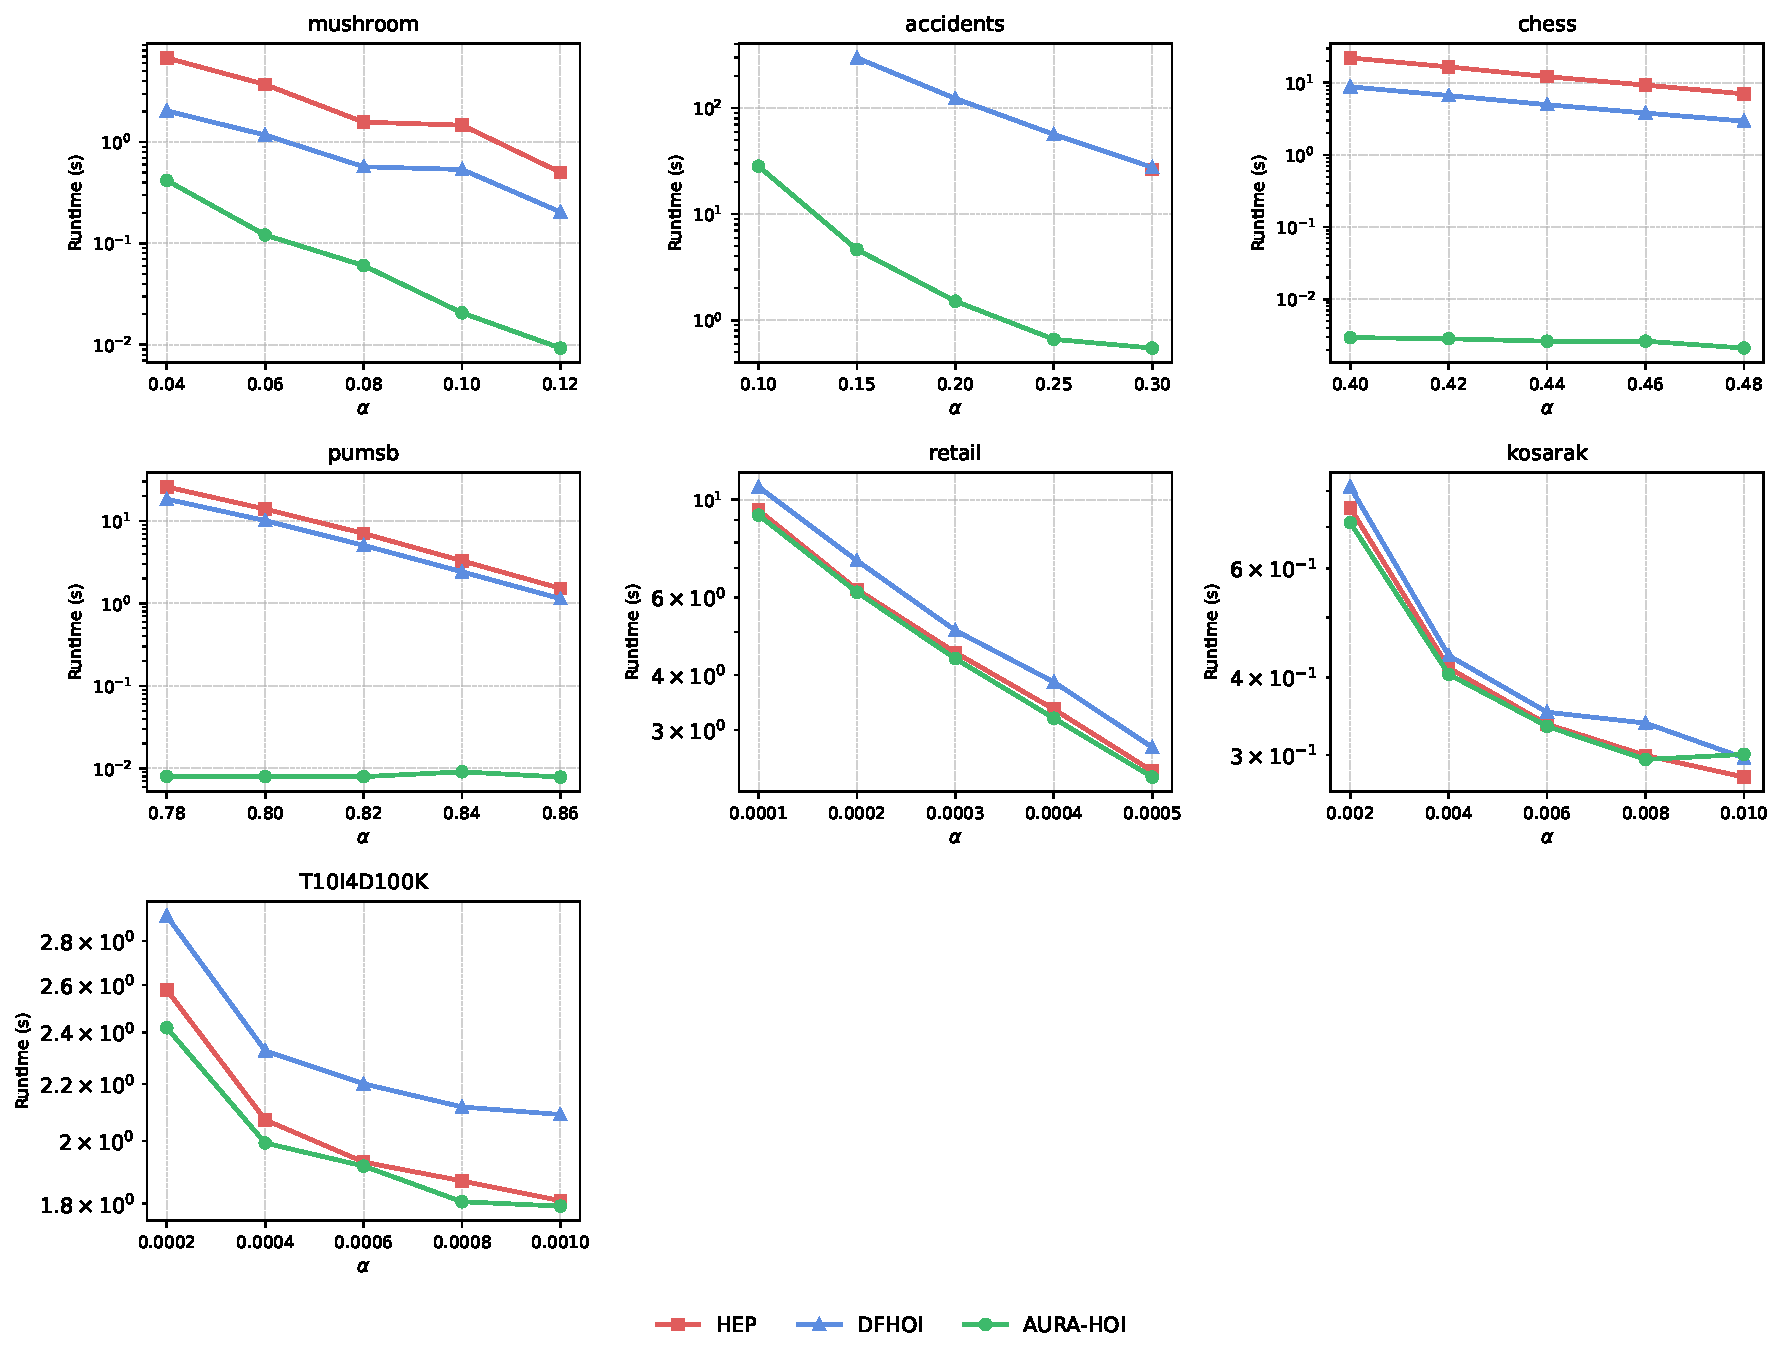
\includegraphics[width=\linewidth]{figures/runtime.pdf}
    \end{column}
    \begin{column}{0.48\textwidth}
      \begin{block}{Speedup Breakdown}
        \begin{itemize}
          \item \textbf{On Dense Datasets:}
            \begin{itemize}
              \item \texttt{mushroom}: \AURA{} is $12\times$ to $26\times$ faster than \DFHOI{}.
              \item \texttt{accidents}: $69\times$ to $85.7\times$ faster!
              \item \texttt{chess} \& \texttt{pumsb}: \textbf{$1,400\times$ to $2,989\times$} faster than \DFHOI{}, up to \textbf{$7,518\times$} faster than \HEP{}!
            \end{itemize}
          \item \textbf{Overcoming Baseline Failure:} At $\alpha = 0.10$ on \texttt{accidents}, \DFHOI{} times out ($>600$ s) and \HEP{} crashes ($>20$ GiB RAM). \AURA{} finishes in \textbf{17.8 seconds}!
          \item \textbf{Sparse Datasets:} Speedup ratio remains $1.02\times$--$1.21\times$, confirming no performance overhead.
        \end{itemize}
      \end{block}
    \end{column}
  \end{columns}
\end{frame}

\begin{frame}{RQ3: Peak Memory Footprint}
  \begin{columns}[T]
    \begin{column}{0.48\textwidth}
      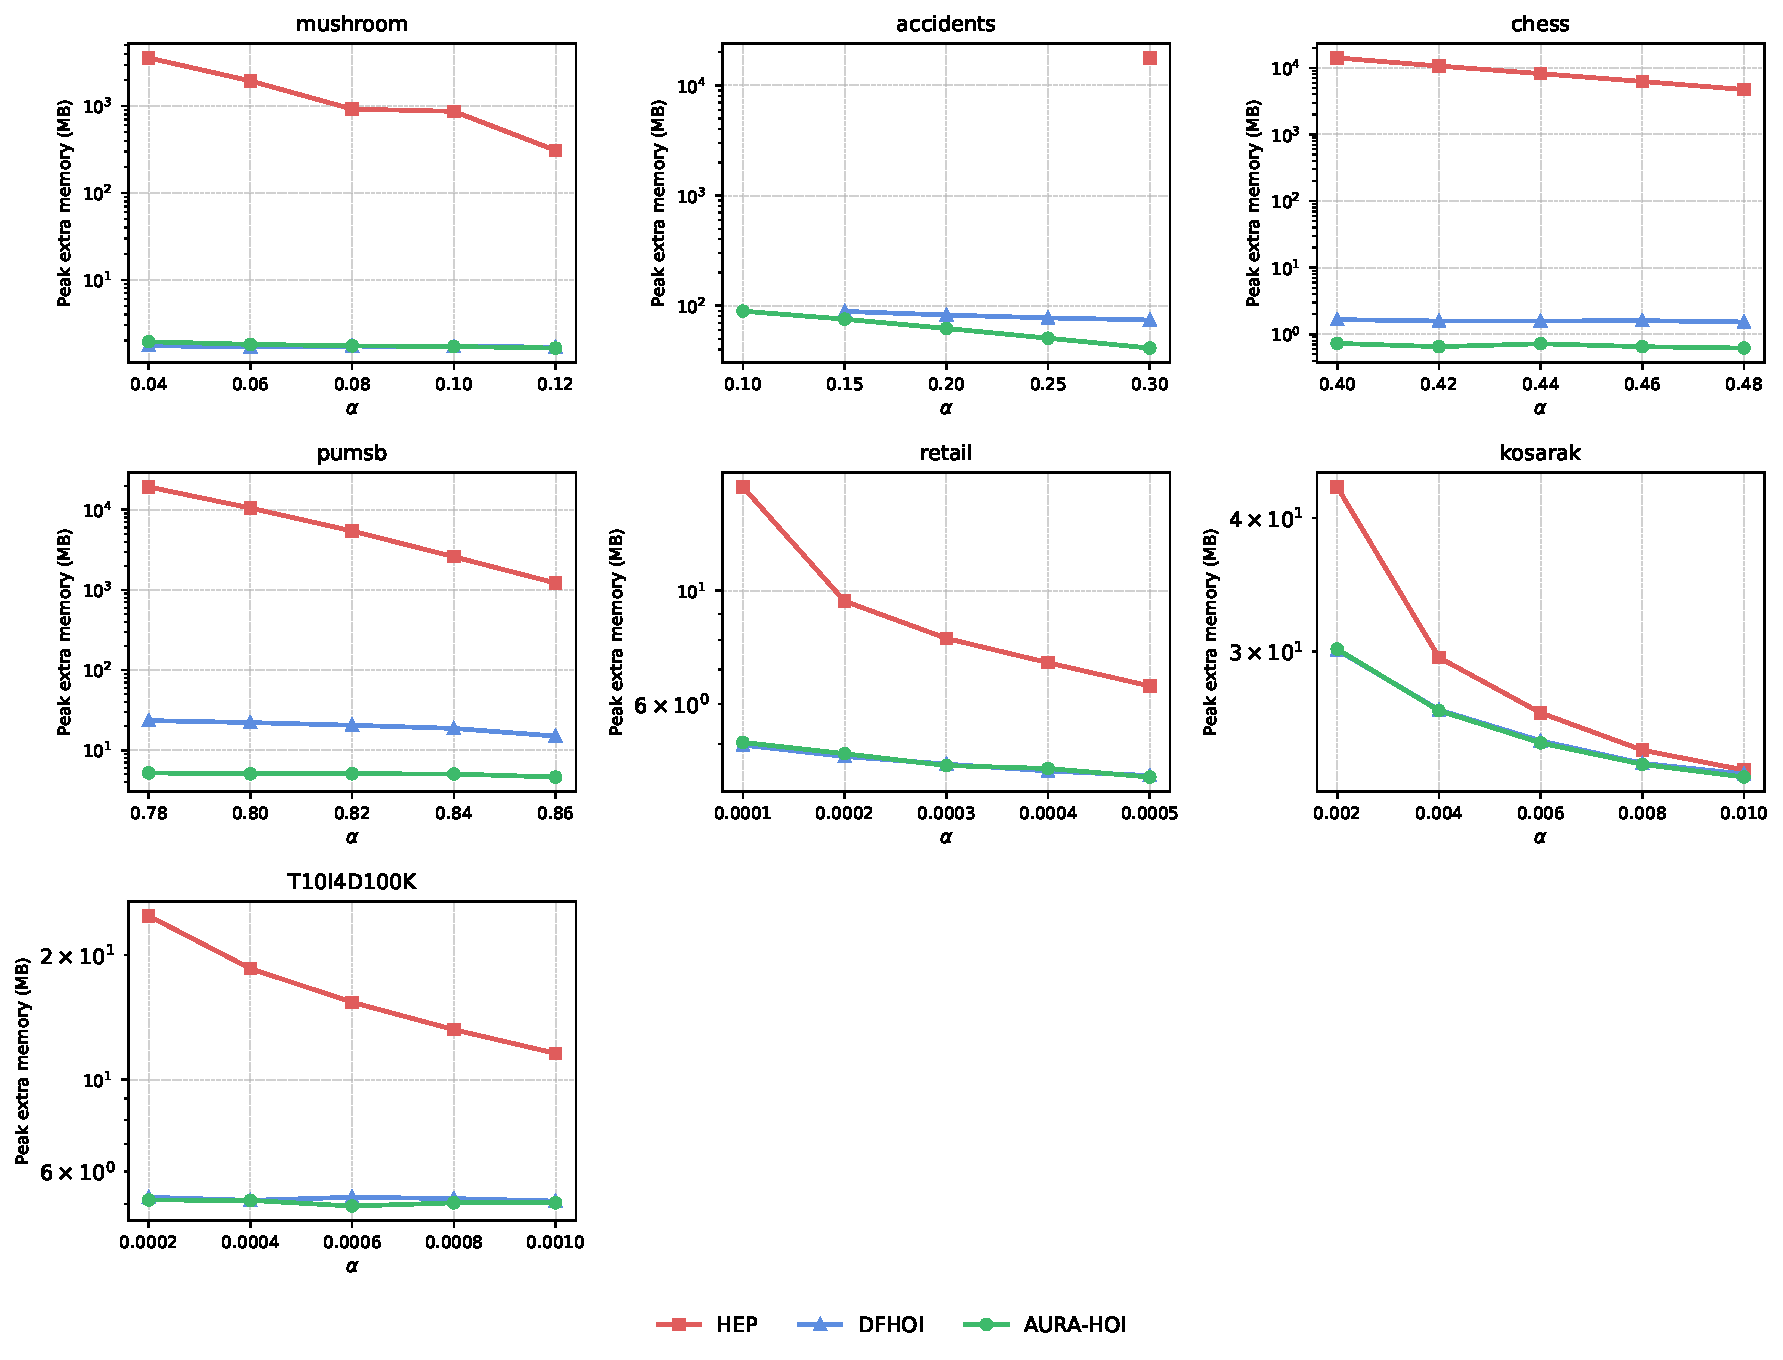
\includegraphics[width=\linewidth]{figures/memory.pdf}
    \end{column}
    \begin{column}{0.48\textwidth}
      \begin{block}{Memory Stability}
        \begin{itemize}
          \item \HEP{} experiences explosive memory growth due to maintaining large candidate structures ($>19.2$ GiB on \texttt{accidents}).
          \item \DFHOI{} requires up to $80$ MB.
          \item \AURA{} peak memory is strictly contained between \textbf{5 MB and 89 MB} across all configurations.
          \item Chunked arena allocator ensures zero memory leaks and predictable, rock-solid heap footprint.
        \end{itemize}
      \end{block}
    \end{column}
  \end{columns}
\end{frame}

\begin{frame}{RQ4: Scalability Analysis}
  \begin{columns}[T]
    \begin{column}{0.48\textwidth}
      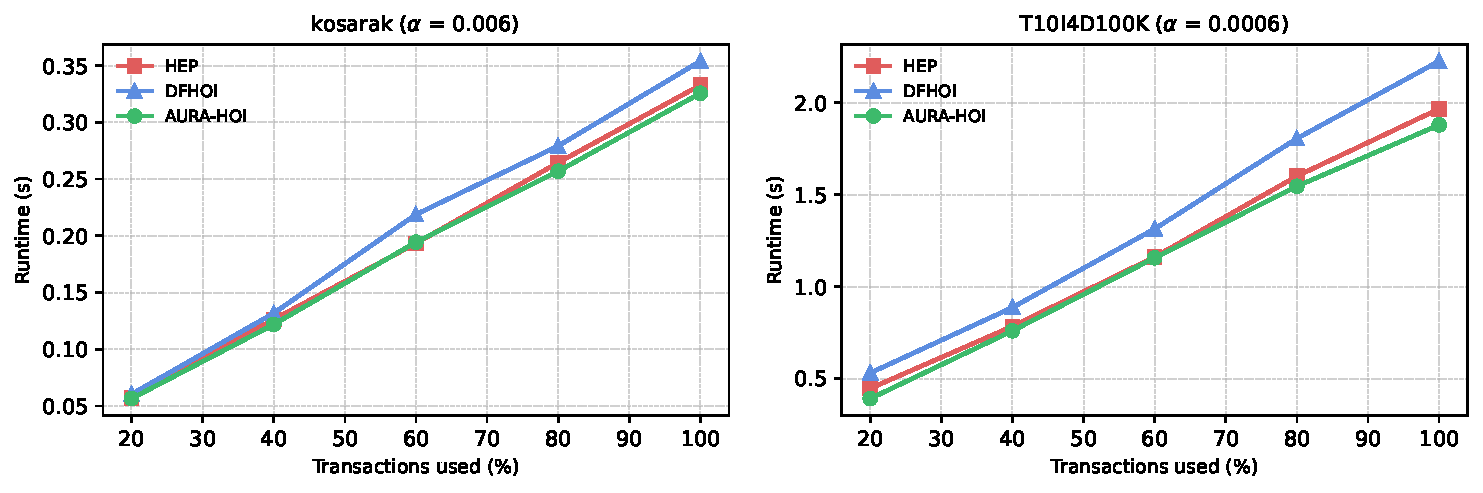
\includegraphics[width=\linewidth]{figures/scalability.pdf}
    \end{column}
    \begin{column}{0.48\textwidth}
      \begin{block}{Linear Scalability with Database Size}
        \begin{itemize}
          \item Tested on prefix slices: 20\%, 40\%, 60\%, 80\%, 100\% of transactions on \texttt{kosarak} and \texttt{T10I4D100K}.
          \item Runtimes grow in direct linear proportion to transaction volume.
          \item Relative ordering (\AURA{} $\approx$ \DFHOI{} $\le$ \HEP{}) remains completely invariant across all data scales.
        \end{itemize}
      \end{block}
    \end{column}
  \end{columns}
\end{frame}

\begin{frame}{Ablation Study: Dissecting Pruning Components}
  \begin{table}
    \small
    \begin{tabular}{llrrrrr}
      \toprule
      Dataset & $\alpha$ & Full \AURA{} & No Tail Cap & No Class Bound & No Residual & No Arena \\
      \midrule
      \texttt{mushroom} & 0.08 & \textbf{0.059 s} & 0.062 s & 0.082 s & 0.425 s & 0.076 s \\
      (Intersections) & & 48,890 & 50,905 & 75,947 & 657,947 & 48,890 \\
      \midrule
      \texttt{accidents} & 0.20 & \textbf{1.47 s} & 1.50 s & 3.47 s & 91.7 s & 1.54 s \\
      (Intersections) & & 1,794 & 1,839 & 6,539 & 482,214 & 1,794 \\
      \bottomrule
    \end{tabular}
  \end{table}

  \begin{block}{Ablation Insights}
    \begin{itemize}
      \item \textbf{No Residual (UBO only):} Intersections surge by \textbf{$13.4\times$} on \texttt{mushroom} and \textbf{$268\times$} on \texttt{accidents}. Runtime increases by $7.2\times$ and $62\times$!
      \item \textbf{No Class Bound:} Intersections increase by $55\%$ on \texttt{mushroom} and $3.6\times$ on \texttt{accidents}.
      \item \textbf{Arena Allocator:} Grants a pure $22\%$ speedup on \texttt{mushroom} by eliminating allocation overhead.
    \end{itemize}
  \end{block}
\end{frame}

% ==============================================================================
% SECTION 5: CONCLUSION & OUTLOOK
% ==============================================================================
\section{Conclusion \& Future Work}

\begin{frame}{Summary of Key Contributions}
  \begin{enumerate}
    \item \textbf{Theoretical Breakthrough:} Formulated the \textbf{Length-Capped Residual Bound} ($\UBres$), proving that search-tree tail limits restrict the maximum achievable occupancy on long transactions.
    \item \textbf{Strict Dominance:} Mathematically proved that $\UBres(X) \le \UBO(X)$ universally, with strict inequality on all dense databases.
    \item \textbf{Closed-Form Evaluation:} Established an $O(1)$ uniform-length closed form that slashes bound evaluation cost to zero.
    \item \textbf{High-Performance Architecture:} Developed an exact rational arithmetic kernel and a chunked arena allocator in native C.
    \item \textbf{Empirical Superiority:} Demonstrated up to \textbf{99.5\%} candidate intersection reduction, up to \textbf{$2,989\times$} speedup over \DFHOI{}, and successfully mined difficult thresholds where baselines failed.
  \end{enumerate}
\end{frame}

\begin{frame}{Future Directions \& Discussion}
  \begin{block}{Open Avenues for Research}
    \begin{itemize}
      \item \textbf{Maximal \& Closed HOIs (MFHOI):} Extending length-capped residual bounds to mine only Pareto-maximal high-occupancy itemsets without redundancy.
      \item \textbf{Per-Transaction Residual Bounds for Sparse Data:} Developing hybrid bounds factoring in transaction-specific item distributions to enhance sparse pruning.
      \item \textbf{Downstream Integration:} Leveraging exact HOIs as compact knowledge primitives for neuro-symbolic recommender systems and clinical pathway discovery.
    \end{itemize}
  \end{block}

  \vspace{0.4cm}
  \begin{center}
    {\Large\textbf{Thank You for Your Attention!}}\\[0.3cm]
    {\normalsize\textbf{Q\&A / Open Discussion}}
  \end{center}
\end{frame}

\end{document}
